\documentclass[a4paper,10pt]{report}
\usepackage[utf8]{inputenc}
\usepackage{hyperref}
\usepackage{graphicx}
\usepackage{float}
% Title Page
\title{Analyse de Comportements avec Twitter}
\author{Antonin Durey Matthieu Caron}




\begin{document}
\pagenumbering{alph}
\maketitle
\clearpage
\pagenumbering{arabic}
\chapter{Description générale du projet}
  \section{Lien vers le git}
    \url{https://github.com/Grimnack/pje2}
  \section{Description de la problématique}
    Le but est de créer une application permettant de tester différents algorithmes
    afin de faire une analyse de sentiments sur Twitter. La problématique est donc la suivante :
    quel est l'algorithme le plus efficace, c'est à dire qui donne le plus souvent la vérité, pour faire de la 
    classification de sentiments ?
  \section{Description générale de l'architecture de votre application}
    Nous avons fait une application java swing. Ainsi, nous avons privilégié une architecture MVC.
    Les modèles contiennent les différentes informations permettant à l'application de fonctionner : les éléments graphiques, les tweets, les éléments de configuration...
    Les vues sont représentés par les différents éléments graphiques de l'application.
    Le contrôle est principalement effectué par la classe Annotation qui s'occupe de classer les tweets en fonction de l'algorithme choisi. 
\chapter{Détails des différents travaux réalisés}
  Le projet se divise en quatre taches majeures, utilisation d'une API twitter afin de récupérer 
  des tweets, préparer une base d'apprentissage afin de ne pas avoir de bruit mais aussi de créer notre 
  base de vérité pour l'apprentissage supervisé. Implémenter et tester différents algorithmes de classification de sentiments et
  enfin pouvoir utiliser ses algorithme depuis une application avec son interface graphique.
  \section{API Twitter}
  % image de l'interface graphique et explication
  \section{Préparation de la base d'apprentissage}
    \subsection{Nettoyage des données}
      Pour nettoyer nos données, nous avons effectué les opérations suivante : 
      \begin{itemize}
       \item Pour les doublons, nous vérifions que les tweets ne sont pas présents en double. Néanmoins, nous considérons qu'un retweet n'est pas un doublon car c'est une manière d'exprimer le même avis que la personne ayant initialement tweeté.
       \item Une option de l'API permet de sélectionner une langue pour les tweets - option que nous avons activé pour s'assurer de ne récupérer que des tweets français.
       \item Nous avons fait un filtrage pour retirer tous les symboles de ponctutation, "RT" signifiant retweet, URL et l'url associée.
      \end{itemize}
      Ce nettoyage comporte plusieurs problèmes. Ne pas considérer que les retweets sont des doublons peut s'avérer problématique. De plus, retirer tous les symboles de ponctuation est très risqué quant à l'interprétation de certaines données. Par exemple, '11.5Mds' devient '115Mds' après avoir appliqué le filtre.
      

    \subsection{Construction de la base}
      Pour construire notre base de tweets, nous le faisons directemment depuis notre application. Nous récupèrons un nombre de tweet paramétrable. En cliquant sur \emph{Etiquetage}, il est par la suite possible d'affecter une classe à un tweet. Enfin, la sauvegarde dans un fichier permet de créer une nouvelle base, ou d'ajouter des tweets dans une base.

  \section{Algorithme de classification}
    Pour tester les différents algorithmes nous avons d'une part regardé s'il y a une forte différence entre la classe qu'un humain affecterait à un tweet et ce que trouve l'algorithme. D'autre part, nous avons analysé le temps de calcul. Nous avons en effet pensé que c'était un facteur très important dans le domaine de la bigdata, même si avions peu de données.
     
    \subsection{mots clefs}
      Pour l'algorithme des mots clefs, nous avons gardé le dictionnaire de mots intact.
      Après analyse, nous avons constaté que 64\% des tweets étaient classés correctement par l'algorithme des mots clefs.
      Pour ce qui est du temps de calcul %%TODO chercher la valeur de la complexité
      
      
    \subsection{KNN}
    
      
    \subsection{Bayes}
      Bayes a été utilisé dans notre programme pour nous permettre d'estimer la classe des tweets qui vont être ajoutés dans notre base. Ainsi, si l'algorithme de Bayes est bien implémenté et qu'il y a une base conséquence de données, il devient possible d'inclure des tweets dans la base grâce à cet algorithme.
      Néanmoins, il est difficile pour un algorithme d'estimer la classe d'un tweets seulement en regardant mot après mot. C'est pourquoi nous avons ajouté plusieurs paramètres dans notre application :
      \begin{itemize}
	    \item Il est possible d'exclure les mots de moins de n lettres - n étant configurable. Cela permet de ne pas prendre en compte les petits comme les articles, pronoms ou déterminants qui n'offrent que peu de sens et qui ne sont généralement pas significatifs pour classifier un tweet. 
	    \item En prenant un thème donné - la SNCF -, il est logique que certains mots ou groupe de mots soient très important pour juger de la classe d'un tweet. Dans le cas de la SNCF, des ensembles de mots tels que \textit{en retard, à l'heure, train annulé...} sont importants et doivent être davantage pris en compte. Dans l'application, cela est représenté par les \textit{n-grammes}.
      \end{itemize}
      De plus, nous laissons le choix de lancer l'algorithme de Bayes en comptant les mots selon leur présence ou selon leur fréquence.
      Nous nous en sommes rendus compte par la suite : dans le cas d'un tweet où le nombre de mots est réduit, ce changement n'apporte pas beaucoup de différence.
  \section{Interface graphique}
    \subsection{copie d'ecran}
      \begin{figure}[H]
	\centering
	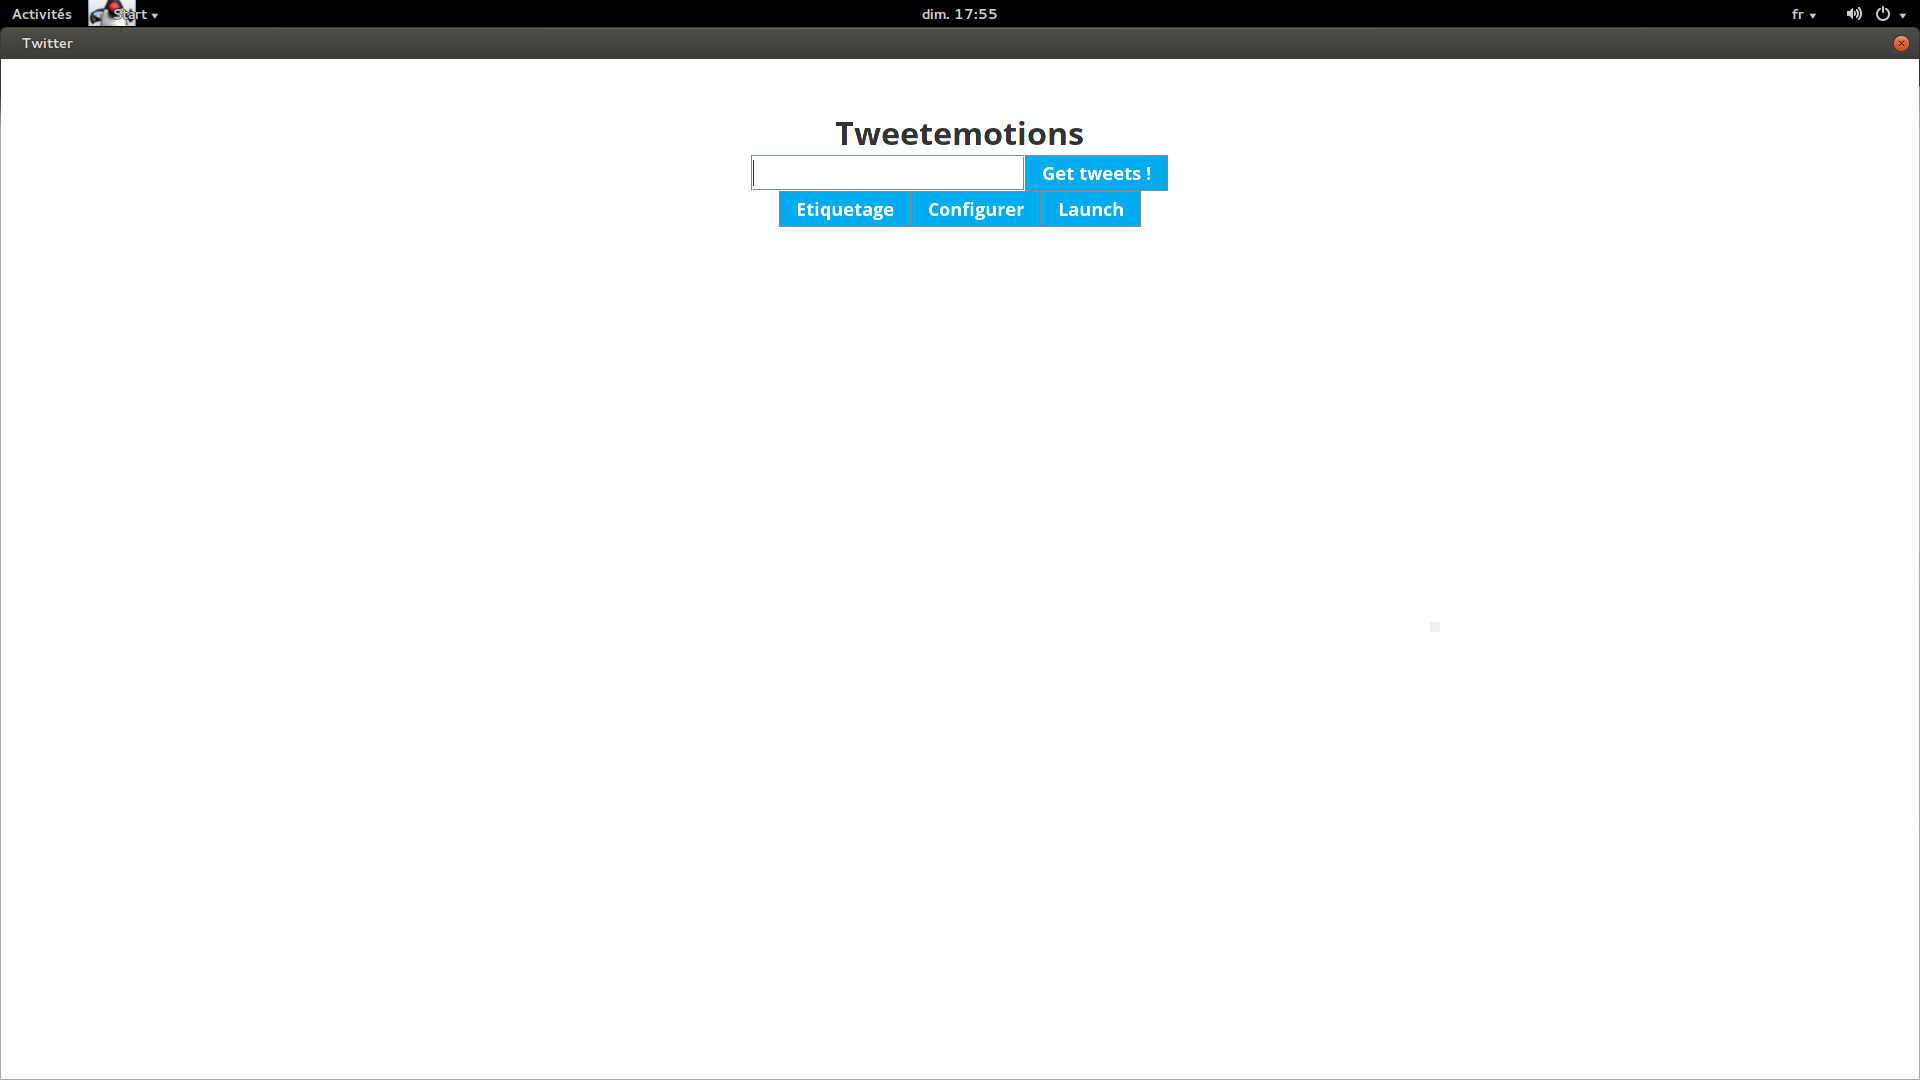
\includegraphics[scale=0.2]{impressions-ecran/accueil.png}
	\caption{Page d'accueil}
	\label{accueil}
      \end{figure}
      \begin{figure}[H]
	\centering
	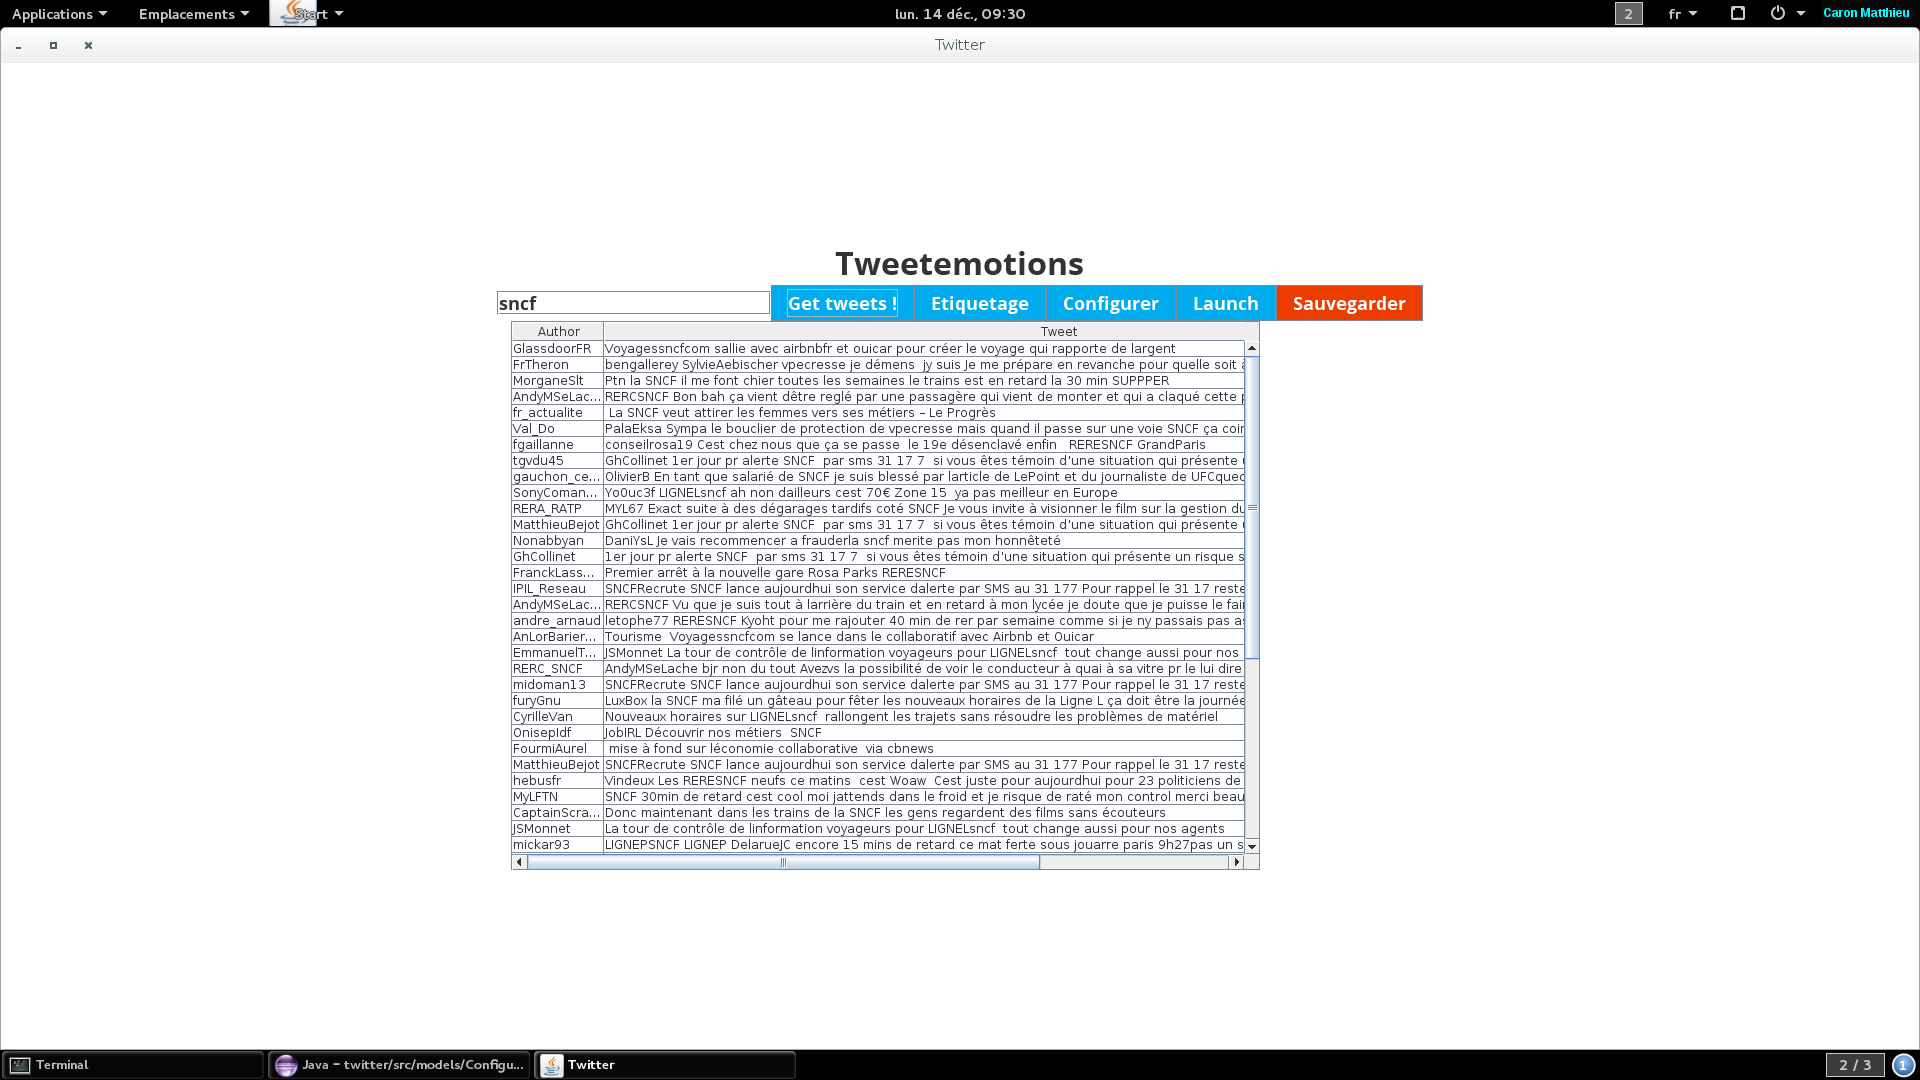
\includegraphics[scale=0.2]{impressions-ecran/tweets.png}
	\caption{Affichage des tweets}
	\label{tweets}
      \end{figure}
      \begin{figure}[H]
	\centering
	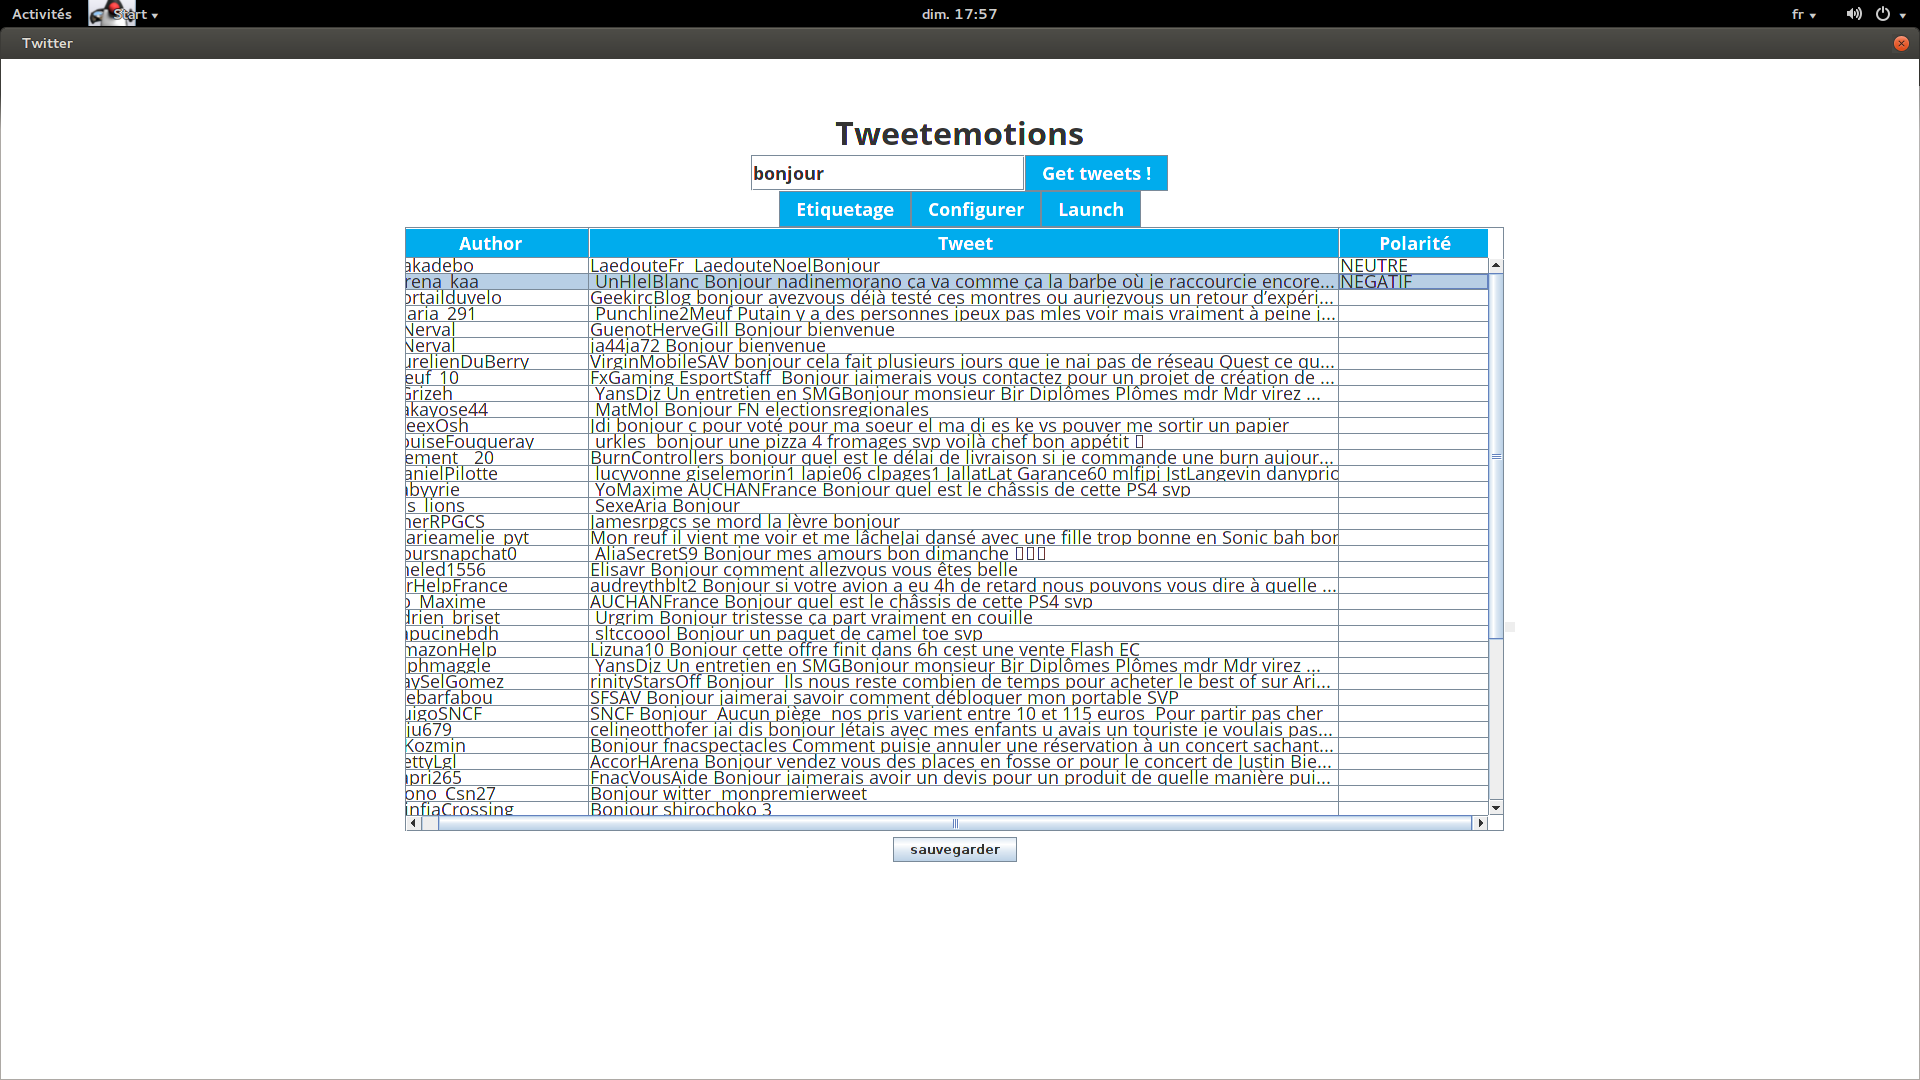
\includegraphics[scale=0.2]{impressions-ecran/etiquetage.png}
	\caption{Étiquetage des tweets}
	\label{etiquetage}
      \end{figure}
      \begin{figure}[H]
	\centering
	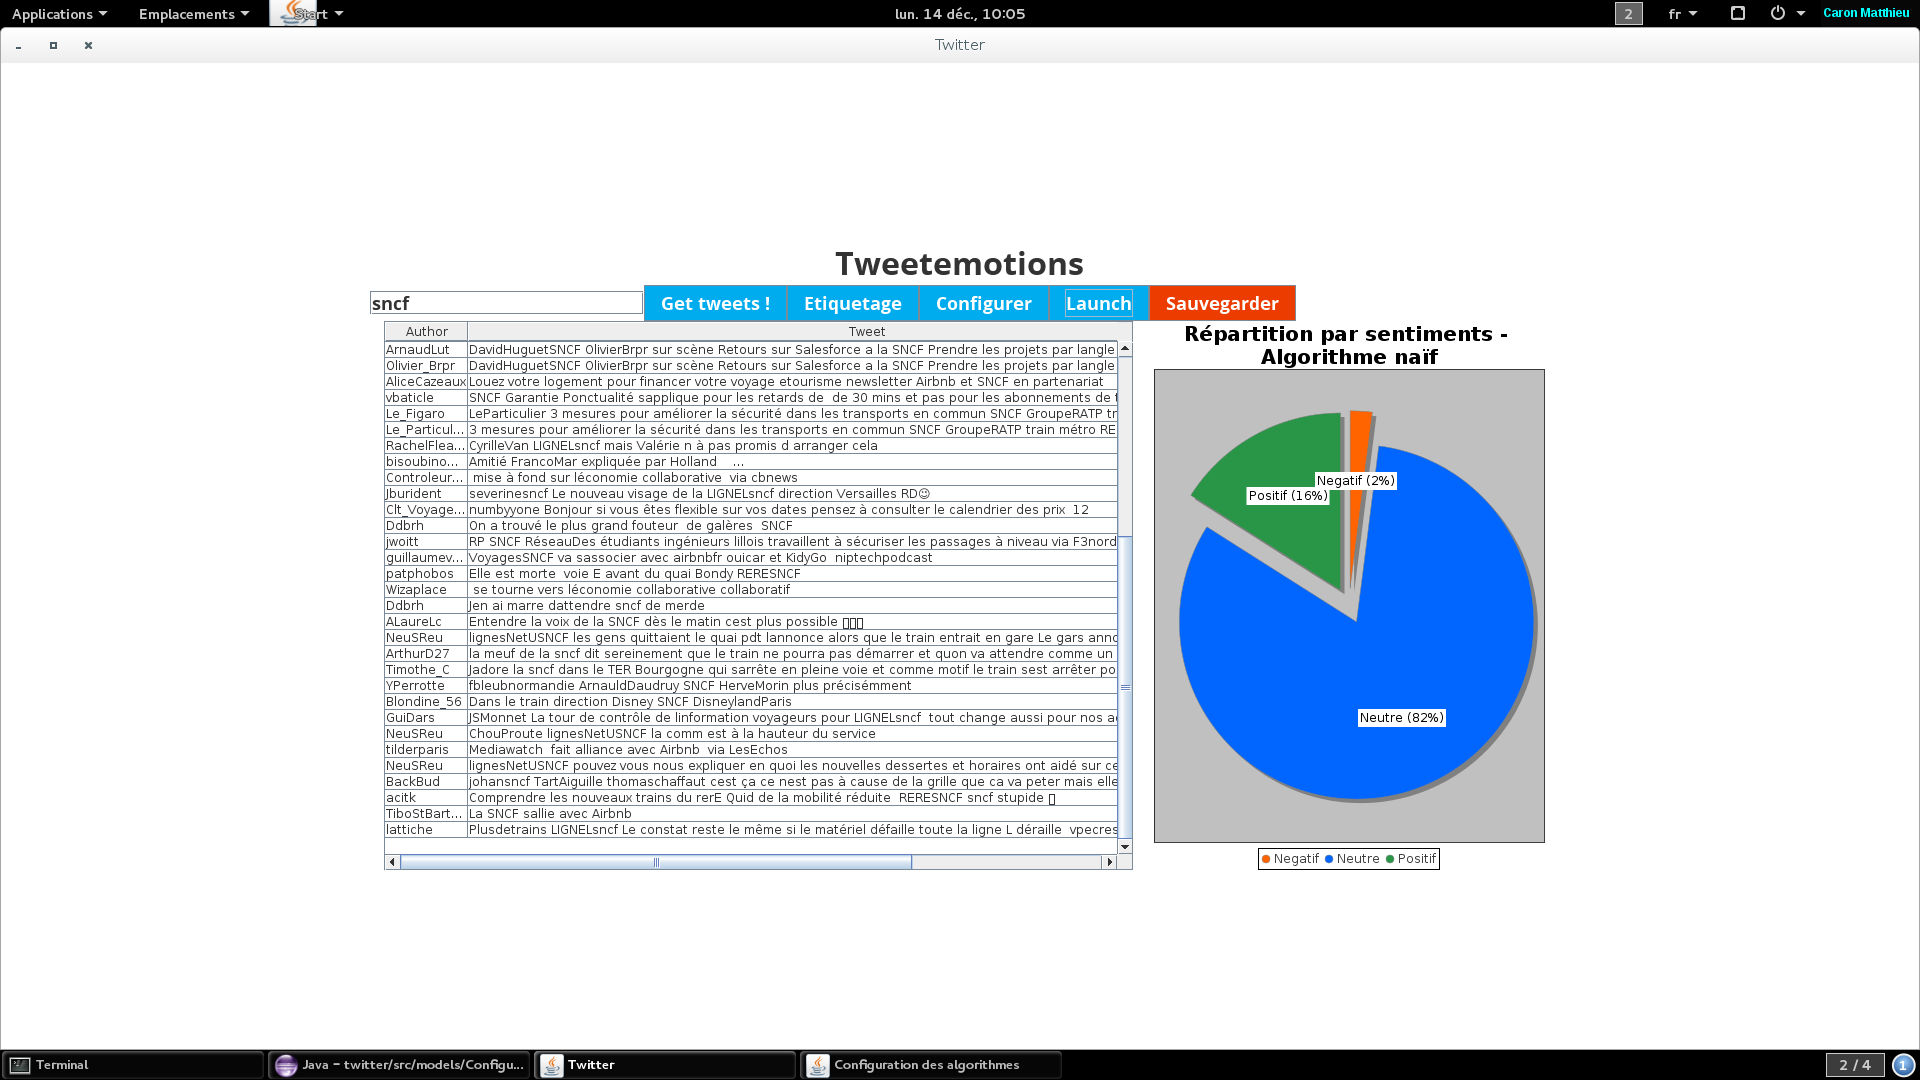
\includegraphics[scale=0.2]{impressions-ecran/dico.png}
	\caption{Algorithme naif}
	\label{dico}
      \end{figure}
      \begin{figure}[H]
	\centering
	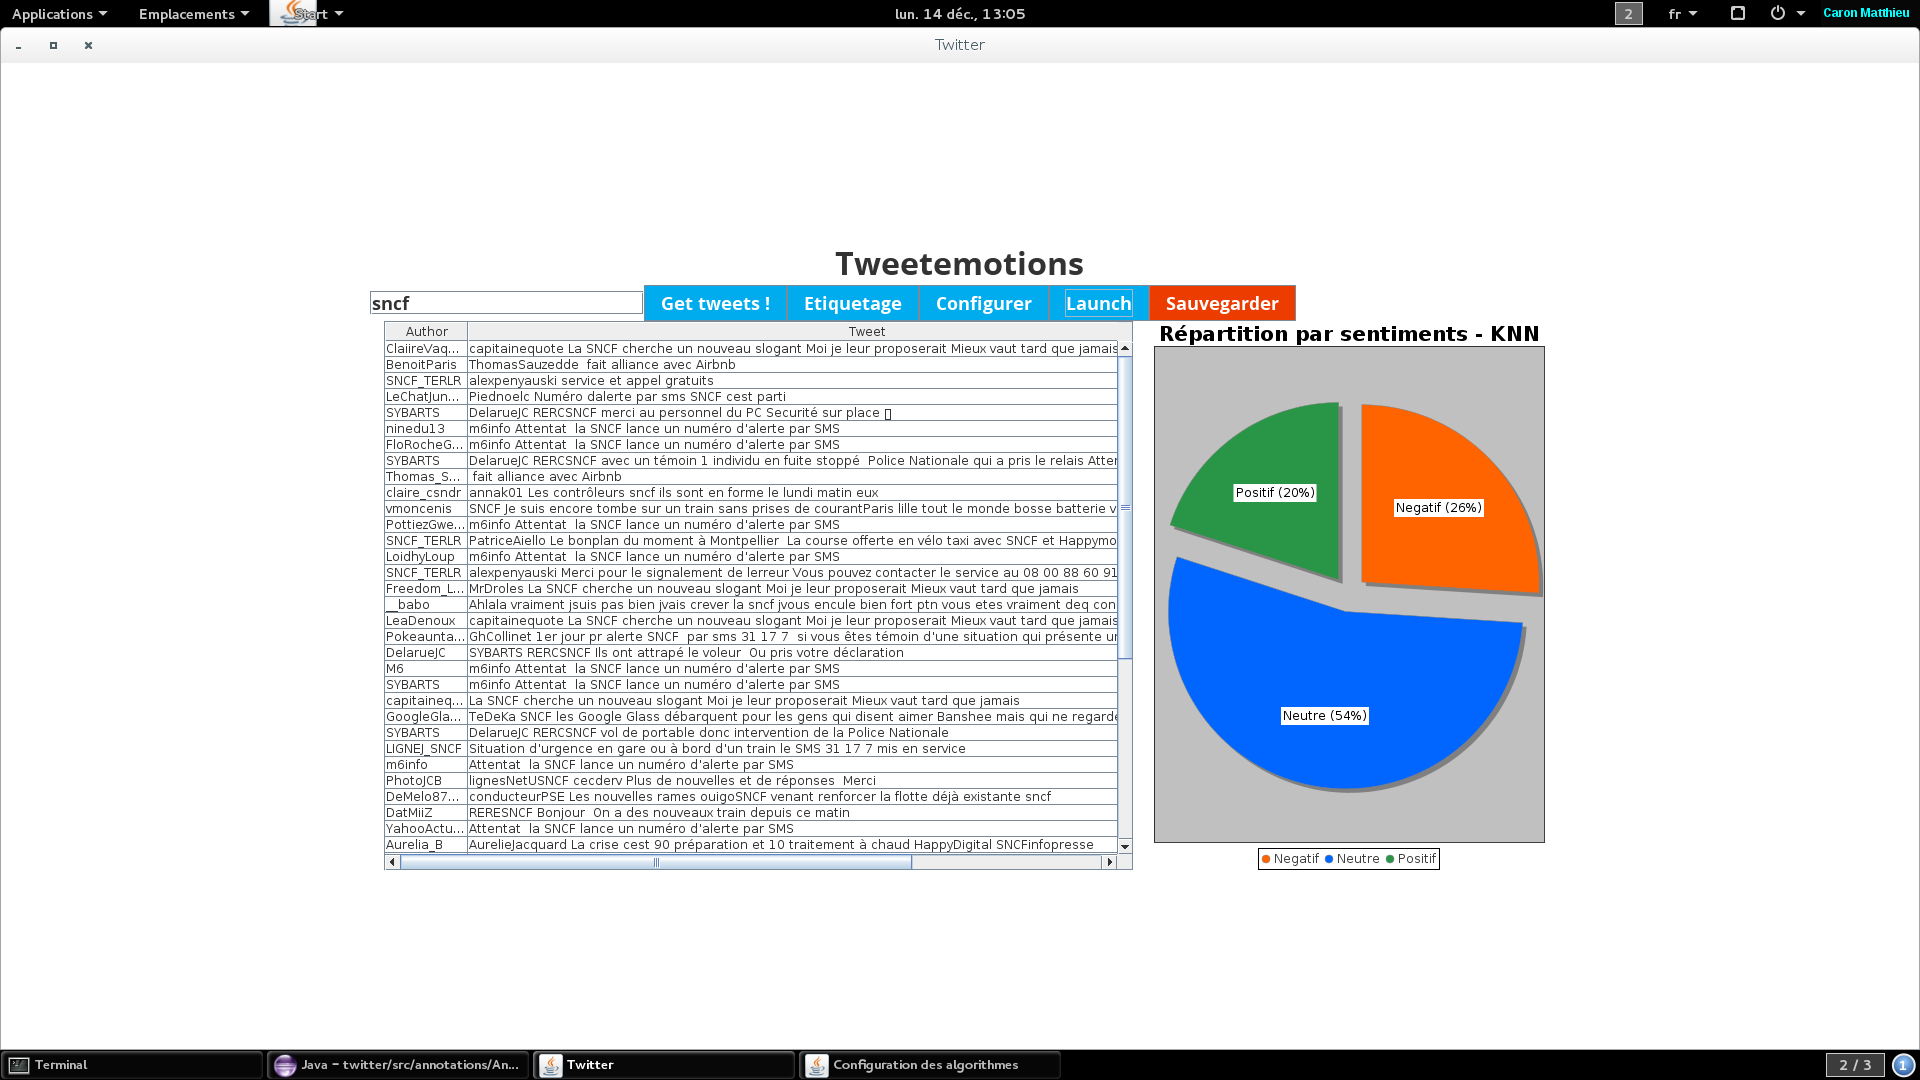
\includegraphics[scale=0.2]{impressions-ecran/KNN.png}
	\caption{Algorithme du plus proche voisin}
	\label{KNN}
      \end{figure}


    
    \subsection{manuel d'utilisation}
      On lance l'application, la fenetre principale est composée d'un champ de texte, un bouton ``get tweets'', un bouton ``Etiquettage'', un bonton ``Configurer'' et 
      un bouton ``Launch''.
      \subsubsection{Le bouton ``Get Tweets''}
	Si vous cliquez sur le bouton ``Get Tweets'', l'application va vous demander combien de tweets vous souhaitez récupérer. Une fois le nombre de tweet choisit,
	il va chercher les tweets contenant la chaine de caractère écrite au préalable dans le champ de texte et va afficher ces tweets à l'écran.
	À partir de ce moment tous les calculs (dico, knn et bayes) se feront sur ces tweets.
      \subsubsection{Le bouton ``Etiquetage''}
	Ce bouton est utile pour ajouter des tweets à une base de données, il faut avoir au préalable cherché des tweets avec le bouton ``Get Tweets''.
	A côté de chaque tweet vous allez devoir choisir qu'elle est leur polarité, neutre, positif ou négatif. Une fois ceci fait pour tous les tweets, vous 
	allez pouvoir sauvegarder vos tweets étiquetés. Pour la sauvegarde un selecteur de fichiers s'ouvre, si vous choisissez un fichier de type .base existant
	les tweets annotés vont être ajouté a la base de tweets choisit. Vous pouvez aussi créer une nouvelle base, il est préférable de choisir l'extension .base
	pour se retrouver dans ses fichiers.
      \subsubsection{Le bouton ``Configurer''}
	Ce bouton sert a choisir l'algorithme de classification entre Dico, KNN et Bayes.On peut aussi choisir si on utilise ou pas le proxy de lille 1, enfin on peut charger une base de tweets depuis
	le menu Configurer.
\chapter{Résultats de la classification avec les différentes méthodes et analyse}
\chapter{Conclusions}
Il faut prendre les resultats des sondages de sentiments avec des pincettes, puisque la réponse affichée à l'écran ne répond pas à 
est-ce que les gens sont pour ou contre tel sujet, mais plutot combien de tweets contenant tel sujet sont positif ou negatif. 



\end{document}     
